Please note that the deadline will be strictly enforced. There will be a $20\%$ penalty if you miss the deadline, with an additional $20\%$ once another 24-hour period elapses. Remember to work alone on this homework; submit everything as a hand-written assignment, except if otherwise indicated.

\vspace{15pt}

\textbf{Instruction}

\begin{enumerate}[label={\arabic*.}]
  \item Go to \url{https://www.overleaf.com} and sign in (required).
  \item Open \href{https://www.overleaf.com/read/qhfsxjjmrpcs}{template}, click \emph{Menu} (up left corner), then \emph{Copy Project}.
  \item Go to \verb|LaTeX/meta.tex| (the file \verb|meta.tex| under the folder \verb|LaTeX|) to change the section and your name, e.g.,
    \begin{itemize}
      \item change title to \verb|\title{MATH 3340-01 Scientific Computing Homework 1}|
      \item change author to \verb|\author{Albert Einstein}|
    \end{itemize}
  \item For Problem 1, 2, 4, 5, you are encouraged to type solutions in \LaTeX{}. But if you want to write it on the printout, make sure your scanned work is \emph{clear} enough, and compile all solutions \emph{in order}, i.e., 1, 2, 3, in a single PDF (failure to do so will lead to points deduction).
  \item For Problem 3, you need to write script files. Here are suggested names for script files:
    \begin{table}[!hbtp]
      \centering
      % \caption{caption}
      % \label{tab:label}
      \begin{tabular}{cllll}
        \toprule
        Problem & Script File         \\
        \midrule
        3(a)    & \verb|hw1_p3_ex1.m| \\
        3(b)    & \verb|hw1_p3_ex2.m| \\
        3(c)    & \verb|hw1_p3_ex3.m| \\
        3(d)    & \verb|hw1_p3_ex4.m| \\
        \bottomrule
      \end{tabular}
    \end{table}

    Once finished, you need to upload these files to the folder \verb|src| on Overleaf. If you have different filenames, please update the filenames in \verb|\lstinputlisting{../src/your_script_name.m}| accordingly. You can code in the provided files in \href{https://libaoj.in/courses/2021s/MATH3340/Homework/1/hw1.zip}{hw1.zip}.
  \item Recompile, download and upload the generated PDF to WyoCourses.
  \item You may find \href{https://libaoj.in/files/LaTeX.Mathematical.Symbols.pdf}{\LaTeX{}.Mathematical.Symbols.pdf} and the second part of \href{https://libaoj.in/courses/2021s/MATH3341/slides/Math.3341.Lab.01.Slides.pdf}{Lab 01 Slides}, and \href{https://libaoj.in/courses/2021s/MATH3341/slides/Math.3341.Lab.02.Slides.pdf}{Lab 02 Slides} helpful.
\end{enumerate}

\newpage

\section{Problem 1}%
\label{sec:problem_1}
Do Ex. 1, Ex. 2 and Ex. 3 on page 16 in the lecture notes. The calculations in these exercises are to be done without the use of MATLAB (although you may use MATLAB to check your answers). Print all your work cleanly and in an organized fashion. This should include explanation at key steps (elaborate in your own words, as appropriate) and general forms of any formulae you're using.
\begin{enumerate}
  \item (Ex. 1) Compute the dot product $\mathbf{x}^{T} \mathbf{y}$ and the inner products $(\mathbf{x}, \mathbf{y})$ and $(\mathbf{x}, \mathbf{x})$ for the two vectors defined by:
    \begin{equation*}
      \mathbf{x} = \begin{bmatrix}
        1 - i \\
        2 \\
        3 + 2i \\
        4i
      \end{bmatrix}, \quad
      \mathbf{y} = \begin{bmatrix}
        2i \\
        -1 \\
        2 - 3i \\
        1 + i \\
      \end{bmatrix}.
    \end{equation*}
  \item (Ex. 2) Find the eigenvalues of the diagonal matrix $D$ given by:
    \begin{equation*}
      D = \begin{bmatrix*}[r]
        2 & 0 \\
        0 & -5 \\
      \end{bmatrix*}.
    \end{equation*}
    Generalize to the case of a diagonal matrix of order $n$.
  \item (Ex. 3) Calculate $A \mathbf{x}$ and $AB$ for the quantities given below. Is the product $BA$ equal to $AB$?
    \begin{equation*}
      A = \begin{bmatrix*}[r]
        2  & 1 & 2 \\
        -1 & 1 & 3 \\
        -2 & 3 & 5 \\
      \end{bmatrix*}, \quad
      B = \begin{bmatrix}
        1 & 2 & 1 \\
        3 & 7 & 2 \\
        3 & 3 & 5 \\
      \end{bmatrix}, \quad
      \mathbf{x} = \begin{bmatrix}
        2 \\
        1 \\
        3 \\
      \end{bmatrix}.
    \end{equation*}
    Then compute the \emph{outer product} $X$ of $\mathbf{x}$ with itself; it is defined by $X = \mathbf{x} \mathbf{x}^{T}$.
\end{enumerate}
%%%%%%%%%%%%%%%%%%%%%%%%%%%%%%%%%%%%%%%%%%%%%%%%%%%%%%%%%%%%%%%%%%%%%%%%%%%%%%%%%%%%%%%%%%%%%%%%%%%%
% Type your solution below
%%%%%%%%%%%%%%%%%%%%%%%%%%%%%%%%%%%%%%%%%%%%%%%%%%%%%%%%%%%%%%%%%%%%%%%%%%%%%%%%%%%%%%%%%%%%%%%%%%%%
\begin{solution}
  \quad
  % \begin{enumerate}
  %   \setlength\itemsep{25em}
  %   \item
  %   \newpage
  %   \item
  %   \item
  %     \quad \vfill
  % \end{enumerate}
  \lstinputlisting[style=Plain]{../src/hw1_sol_p1.txt}
\end{solution}

\section{Problem 2}%
\label{sec:problem_2}
Calculate the product $C = AB$ of the two matrices $A$ and $B$ given below. For each entry in the product matrix show how all the pertinent calculations, i.e. write out clearly the sums and products involved.
\begin{equation*}
  A = \begin{bmatrix*}[r]
    2  & -3 & 1 & 7 \\
    -1 & 3  & 5 & -2 \\
    1  & -1 & 4 & 2 \\
  \end{bmatrix*}, \quad
  B = \begin{bmatrix*}[r]
    3  & 2 \\
    1  & -1 \\
    4  & 1 \\
    -2 & 5 \\
  \end{bmatrix*}.
\end{equation*}
%%%%%%%%%%%%%%%%%%%%%%%%%%%%%%%%%%%%%%%%%%%%%%%%%%%%%%%%%%%%%%%%%%%%%%%%%%%%%%%%%%%%%%%%%%%%%%%%%%%%
% Type your solution below
%%%%%%%%%%%%%%%%%%%%%%%%%%%%%%%%%%%%%%%%%%%%%%%%%%%%%%%%%%%%%%%%%%%%%%%%%%%%%%%%%%%%%%%%%%%%%%%%%%%%
\begin{solution}
  % \quad \vfill % DELETE THIS LINE IF YOU ARE TYPING THE SOLUTION
  \quad
  \lstinputlisting[style=Plain]{../src/hw1_sol_p2.txt}
\end{solution}

\section{Problem 3}%
\label{sec:problem_3}
Do Ex. 1 through Ex. 4 on page 41 (at the end of chapter 3) in the lecture notes. For each of these problems you should submit the code snippet that performs the task, as well as the output. Use a separate scripts or functions each time.
\begin{enumerate}
  \item (Ex. 1) Write a MATLAB function that, given a positive integer $n$, checks whether the sum $S(n)$ defined by
    \begin{equation*}
      S(n) = \sum_{k = 1}^{n} \frac{1}{k (k + 2)}.
    \end{equation*}
  satisfies $S(n) < 3/4$ for all positive integers less than or equal to $n$. The function should take an integer $n$ as input, which can be created in MATLAB with the \verb|colon| operator, and return a vector of exactly $n$ boolean values as output. Check your code by calling the function with several values of $n$.
  \item (Ex. 2) Create an anonymous MATLAB function that computes the value of $f(x)$, defined piecewise as:
    \begin{equation*}
      f(x) = \begin{cases}
        x + 1   & x \leq 0, \\
        \sin(x) & x > 0.
      \end{cases}
    \end{equation*}
  \item (Ex. 3) Write a MATLAB anonymous function that can be used to compute an approximation to $e^{x}$ using the first five terms of the Taylor series for the exponential around the point $x = 0$, that is:
    \begin{equation*}
      e^{x}
      \approx 1 + x + \frac{x^{2}}{2!} + \frac{x^{3}}{3!} + \frac{x^{4}}{4!}.
    \end{equation*}
    For a given point $x$, define the error in the approximation by calculating the absolute value of the difference $|f(x) - e^{x}|$. Plot this error versus $x$ for all the points in the MATLAB vector \verb|x = 0:0.2:2|.
  \item (Ex. 4) Use the MATLAB help system to learn about the function \verb|isprime|, then use this function together with \verb|find| and the colon operator to produce a list of all the prime numbers less than or equal to $M = 30$.
\end{enumerate}
\begin{solution}
  \quad
  \begin{enumerate}
    \item MATLAB script: \lstinputlisting[style=MATLAB]{../src/hw1_p3_ex1.m}
    \item MATLAB script: \lstinputlisting[style=MATLAB]{../src/hw1_p3_ex2.m}
    \item MATLAB script: \lstinputlisting[style=MATLAB]{../src/hw1_p3_ex3.m}
    \item MATLAB script: \lstinputlisting[style=MATLAB]{../src/hw1_p3_ex4.m}
    % \newpage \quad \vfill
  \end{enumerate}
  \lstinputlisting[style=Plain]{../src/hw1_sol_p3.txt}
  \begin{figure}[!hbtp]
    \centering
    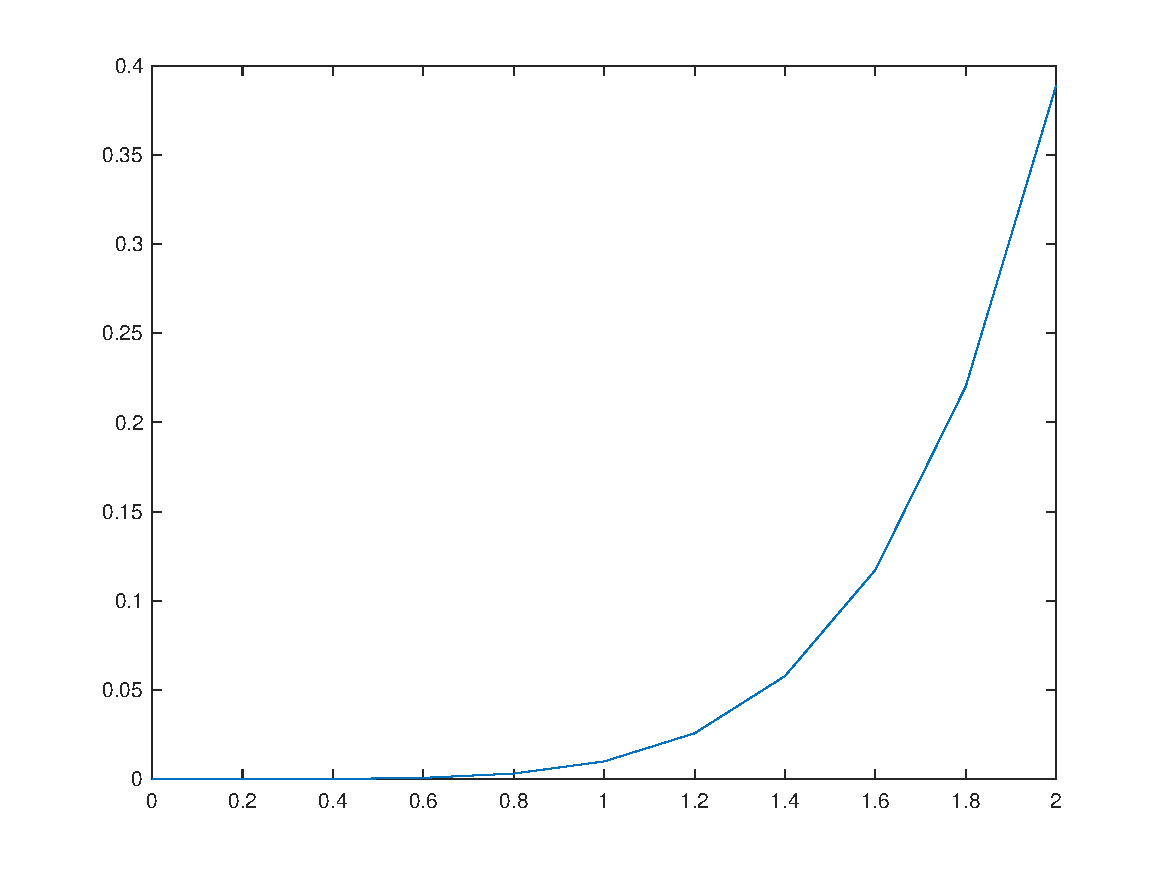
\includegraphics[width=0.75\linewidth]{../src/hw1_p3_c.pdf}
  \end{figure}
\end{solution}

\section{Problem 4}%
\label{sec:problem_4}
Convert to base two the following integers and floating-point numbers: $7$, $13$, $7.75$ and $13.25$. Do these calculations by hand, and explain your answers.
%%%%%%%%%%%%%%%%%%%%%%%%%%%%%%%%%%%%%%%%%%%%%%%%%%%%%%%%%%%%%%%%%%%%%%%%%%%%%%%%%%%%%%%%%%%%%%%%%%%%
% Type your solution below
%%%%%%%%%%%%%%%%%%%%%%%%%%%%%%%%%%%%%%%%%%%%%%%%%%%%%%%%%%%%%%%%%%%%%%%%%%%%%%%%%%%%%%%%%%%%%%%%%%%%
\begin{solution}
  \quad \vfill % DELETE THIS LINE IF YOU ARE TYPING THE SOLUTION
\end{solution}

\section{Problem 5}%
\label{sec:problem_5}
Read about integer and floating-point number representation on digital computers. You'll find information on the internet as well as printouts in the class materials. Then answer the following three questions:
\begin{enumerate}
  \item what is the range for an unsigned integer represented on $64$ bits?
  \item what is the range of a signed integer that is represented on $64$ bits?
  \item what is the range of a double precision floating-point number represented using the IEEE-754 standard with a mantissa of 52 digits?
\end{enumerate}
%%%%%%%%%%%%%%%%%%%%%%%%%%%%%%%%%%%%%%%%%%%%%%%%%%%%%%%%%%%%%%%%%%%%%%%%%%%%%%%%%%%%%%%%%%%%%%%%%%%%
% Type your solution below
%%%%%%%%%%%%%%%%%%%%%%%%%%%%%%%%%%%%%%%%%%%%%%%%%%%%%%%%%%%%%%%%%%%%%%%%%%%%%%%%%%%%%%%%%%%%%%%%%%%%
\begin{solution}
  \quad
  % \begin{enumerate}
  %   \setlength\itemsep{12em}  % DELETE THIS LINE IF YOU ARE TYPING THE SOLUTION
  %   \item
  %   \item
  %   \item
  %     \quad \vfill            % DELETE THIS LINE IF YOU ARE TYPING THE SOLUTION
  % \end{enumerate}
  \lstinputlisting[style=Plain]{../src/hw1_sol_p5.txt}
\end{solution}
